% Horizon penetrating coordinates (vs. Schwarzschild coordinates)
% for a black hole spacetime, with excision
% Author: Jonah Miller
\documentclass[tikz,border=0pt]{standalone}
\usepackage{tikz}
\usetikzlibrary{arrows}
\usetikzlibrary{arrows.meta}
\usetikzlibrary{decorations.markings}
\usepackage{pgfplots}
\usepackage{amsmath}
\usetikzlibrary{decorations.pathreplacing}
\usepackage{scalefnt}

\usepackage[utf8]{inputenc}

\usepgfplotslibrary{fillbetween}
\usepackage{lmodern}

%\tikzset{>={Latex[length=3mm]}}

\tikzstyle{mybox} = [draw=black,
    rectangle, inner sep=10pt, inner ysep=10pt]
\tikzstyle{fancytitle} =[fill=blue!30, text=black]

\begin{document}
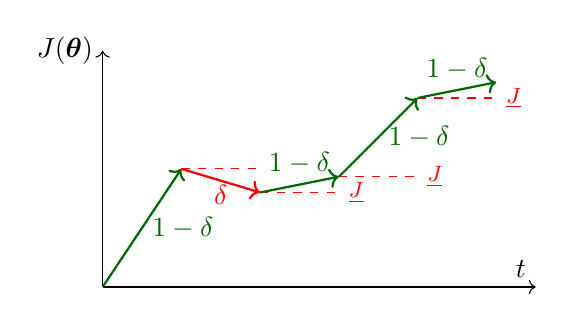
\begin{tikzpicture}[xscale=1]

\draw[->] (0,0) -- (5.5,0) node[above left]{$t$};
\draw[->] (0,0) -- (0,3) node[left]{$J(\boldsymbol{\theta})$};

\draw[thick,->, black!60!green] (0,0) -- (1,1.5) node[midway,right]{$1-\delta$};
\draw[dashed,red] (1,1.5) -- (2,1.5);
\draw[thick,->, red] (1,1.5) -- (2,1.2) node[midway,yshift=-5pt]{$\delta$};
\draw[dashed,red] (2,1.2) -- (3,1.2) node[right]{\footnotesize $\underline{J}$};
\draw[thick,->, black!60!green] (2,1.2) -- (3,1.4) node[midway,above]{$1-\delta$};
\draw[dashed,red] (3,1.4) -- (4,1.4) node[right]{\footnotesize $\underline{J}$};
\draw[thick,->, black!60!green] (3,1.4) -- (4,2.4) node[midway,right]{$1-\delta$};
\draw[dashed,red] (4,2.4) -- (5,2.4) node[right]{\footnotesize $\underline{J}$};
\draw[thick,->, black!60!green] (4,2.4) -- (5,2.6) node[midway,above]{$1-\delta$};


%\draw[dashed,red] (2,1.5) -- (4,0.5);
%\draw[dashed,red] (3,1.2) -- (4,0.5);
%\draw[dashed,red] (5,2.4) -- (4,0.5);
%\draw[dashed,red] (4,1.4) -- (4,0.5) node[fill=white, text=red]{$\underline{J}$};



\end{tikzpicture}
\end{document}